\chapter*{Introduction}
\addcontentsline{toc}{chapter}{Introduction}

Introduce the problem, explain why it is interesting and outline the goal of the thesis.

%%-----------------------------------------------------------------------------------------
%%-----------------------------------------------------------------------------------------
\section*{Morphome3cs}

TODO
%%-----------------------------------------------------------------------------------------
%%-----------------------------------------------------------------------------------------
\section*{Applications of Mesh Difference Visualization}

TODO
%%-----------------------------------------------------------------------------------------
%%-----------------------------------------------------------------------------------------
\section*{Mesh Difference Visualization in Morphome3cs and Elsewhere}

Morphome3cs is able to generate a homologous\footnotemark pair of triangle meshes from two arbitrary triangle meshes and use it to compute and visualize the difference between them. Currently, Morphome3cs is able to produce color-based visualizations of multiple difference metrics. These metrics are:

\begin{itemize}
\item Vertex distance (fig. \ref{fig:morpho_example})
\item Vertex distance projected into the surface normal
\item Angle between corresponding surface normals
\item FESA\footnotemark
\item Curvature difference
\end{itemize}

The disadvantage of these color-based visualizations is that they fail to capture multi-dimensional information. For example, when using vertex distance as a metric, it is impossible to encode both magnitude and direction into color at the same time while maintaining visual clarity.

\begin{figure}[h]
\centering
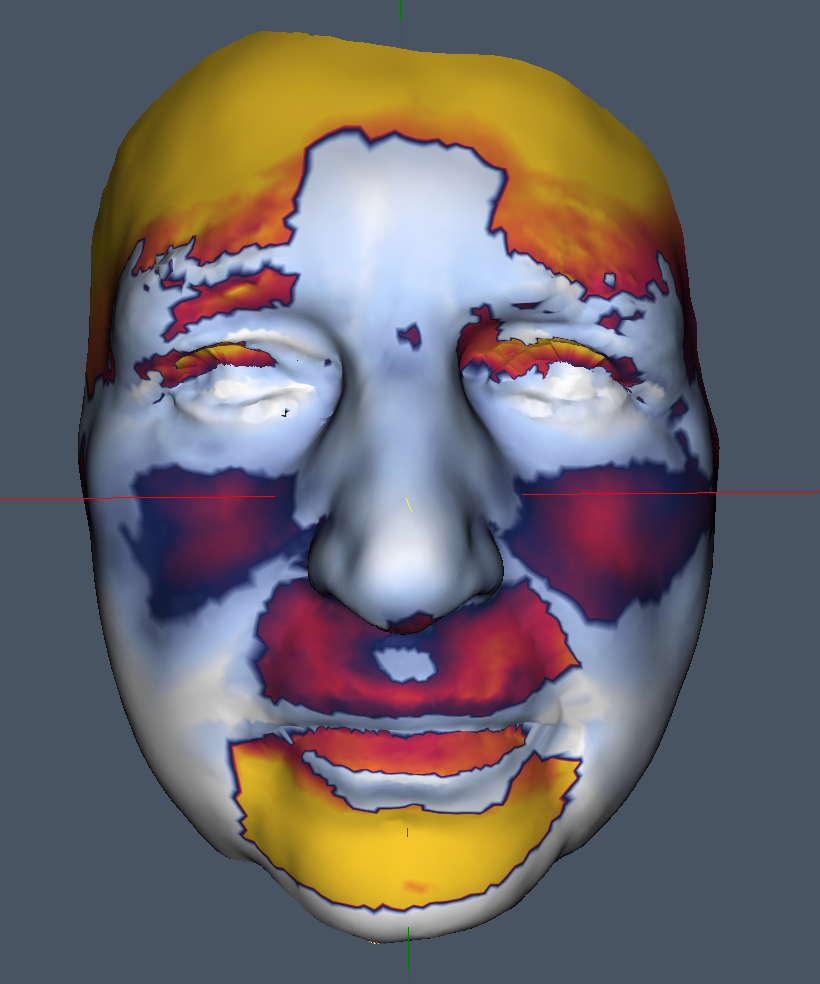
\includegraphics[width=0.5\textwidth]{./img/morpho-example01.PNG}
\caption{Morphome3cs - Vertex difference visualization}
\label{fig:morpho_example}
\end{figure}

Other approaches can be found for example in MeshLab (fig. \ref{fig:meshlab_example}) and CloudCompare (fig. \ref{fig:cloudcompare_example}). Both programs, however, also use only color-based visualizations. Both programs work with arbitrary triangle meshes and CloudCompare can also work with point clouds, register them and visualize the difference between them.

\begin{figure}[h]
\centering
	\begin{subfigure}{0.3\textwidth}
	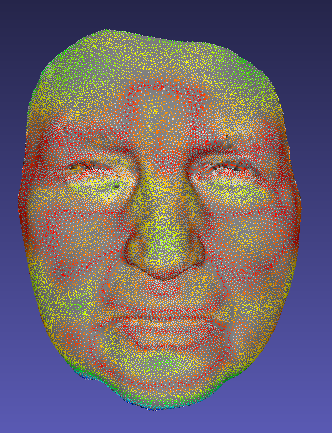
\includegraphics[width=\textwidth]{./img/meshlab-example01.PNG}
    \caption{MeshLab - Hausdorff Distance visualization}
    \label{fig:meshlab_example}
	\end{subfigure}
    \qquad
    \begin{subfigure}{0.3\textwidth}
	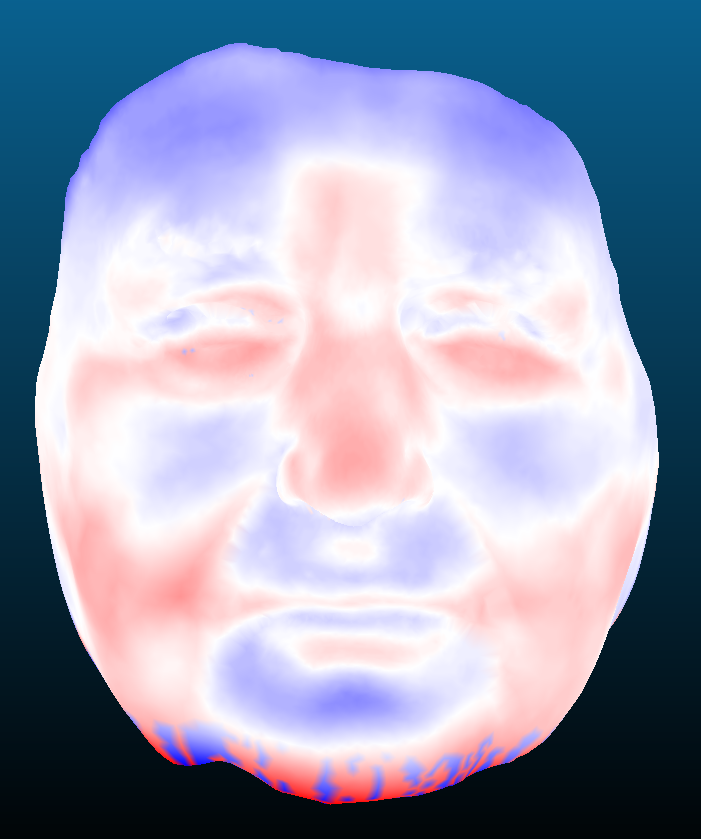
\includegraphics[width=\textwidth]{./img/cloudcompare-example01.PNG}
    \caption{CloudCompare - Vertex distance visualization}
    \label{fig:cloudcompare_example}
	\end{subfigure}
\caption{Visualizations in MeshLab and CloudCompare}
\end{figure}

\addtocounter{footnote}{-2}
\stepcounter{footnote}\footnotetext{Two triangle meshes are homologous if they have the same number of vertices and there is a one-to-one mapping between them. Vertices are numbered and vertex \(v_i \in Mesh_1\) corresponds to vertex \(v_i \in Mesh_2\).}
\stepcounter{footnote}\footnotetext{{\it Finite Element Surface Analysis}, captures the difference between corresponding triangle areas}
%%-----------------------------------------------------------------------------------------
%%-----------------------------------------------------------------------------------------
\section*{Our Goal}

In order to overcome the limitations of the above visualizations, this thesis is looking to create arrow-based visualizations which will be able to display multidimensional information. We will also focus on the visual appearance of devised visualizations and their implementation in an experimental application. Lastly, a user study will be carried out to assess the quality of the new visualizations in various use cases. This study will serve as a basis for further development and potential incorporation of the visualizations into Morphome3cs.
%%-----------------------------------------------------------------------------------------
%%-----------------------------------------------------------------------------------------